\subsection{Crossing forecasts transfer across the tested geometries}
At the primary setting the exact tie direction agreed with the small forward probe on all 7,144 eligible synthetic and 1,007 eligible public top ties. The counts are over accepted pairwise root probes, which may visit the same boundary region. No quantitative claim is made about ties excluded by the derivative or top-gap conditions.

The main query-level result was the improvement in ranking endpoint changes over initial ambiguity (Figure~\ref{fig:forecast} and Table~\ref{tab:rank}). On synthetic units with both outcomes, the projected margin's AP was $0.9966$, versus $0.4846$ for the negative initial margin. The equal-seed difference was $0.5120$ with interval $[0.4911,0.5332]$. The public unit-macro AP values were $0.9867$ and $0.5251$, with an equal-seed difference of $0.4576$ and interval $[0.3798,0.5360]$. These mean APs average the 108 synthetic and 20 public units containing both outcomes, at mean change prevalences 16.42\% and 8.03\%. The four omitted public units and the separated-lobe control had no eligible mixed outcome. Ordinary linear projection reached $0.9849$ and $0.9891$, and exponential Euler reached $0.9954$ and $0.9904$. The comparison supports the use of a one-step directional forecast over static uncertainty. It gives little evidence of a practically meaningful ranking advantage over exponential Euler.

\begin{table}[htbp]
\centering
\small
\caption{Primary regime. AP is averaged over units with both endpoint changes and nonchanges. The final column gives transported minus static balanced accuracy. Labels in the first three AP columns describe forecasts of changes relative to the solver, not class labels.}
\label{tab:rank}
\begin{tabular}{lrrrrr}
\toprule
Family & Mixed units & Initial AP & Projected AP & ETD1 AP & BA shift (pp)\\
\midrule
Affine shells & 36 & .4581 & .9990 & .9994 & $+7.43$\\
Wavy shells & 36 & .5460 & .9995 & .9986 & $-4.77$\\
Open chains & 36 & .4498 & .9915 & .9881 & $-1.06$\\
Separated lobes & 0 & -- & -- & -- & $0.00$\\
PenDigits & 12 & .4839 & .9779 & .9841 & $-2.43$\\
Seeds & 8 & .5869 & 1.0000 & 1.0000 & $-1.79$\\
\bottomrule
\end{tabular}
\end{table}

\begin{figure}[htbp]
\centering
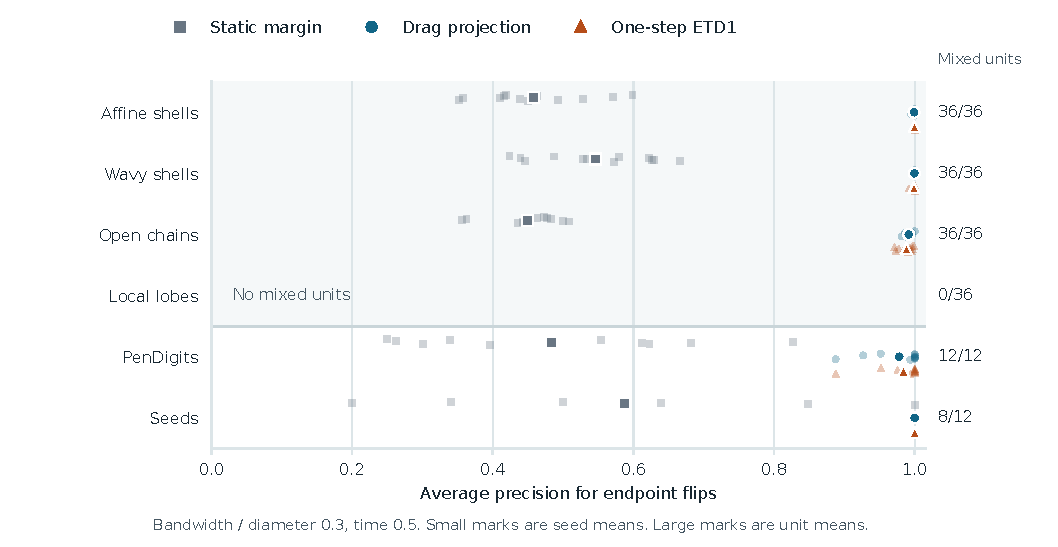
\includegraphics[width=\linewidth]{figures/forecast.pdf}
\caption{Prospective endpoint-change ranking at the primary bandwidth and horizon. Unit-level AP is undefined for units without both outcomes. ETD1 reads the class scores after one exponential Euler step.}
\label{fig:forecast}
\end{figure}

\subsection{Enclosures cover many stable queries and rarely prove a primary-horizon departure}
We observed no certificate contradictions against the numerical reference at any locked setting. At the primary horizon the combination certified the terminal label for 32.08\% of synthetic and 41.62\% of public query units on average. Whole-interval coverage exceeded that of the displacement-only ball by 5.83 percentage points (seed interval $[4.98,6.74]$) and 34.19 points ($[30.91,37.38]$). The combined terminal-label tests exceeded ordinary Taylor coverage by 0.04 and 0.23 points at this setting. Most certificates established preservation. Of 6,383 synthetic and 140 public endpoint changes, just 19 and zero were certified departures at this horizon. At horizon $0.15$ and bandwidth ratio $0.30$, the counts were 700 of 2,090 and 6 of 34. Figure~\ref{fig:certification} shows the dependence on scale and horizon. One primary case in each stage sampled a changed label that later returned. Endpoints alone would miss those cases.

\begin{figure}[htbp]
\centering
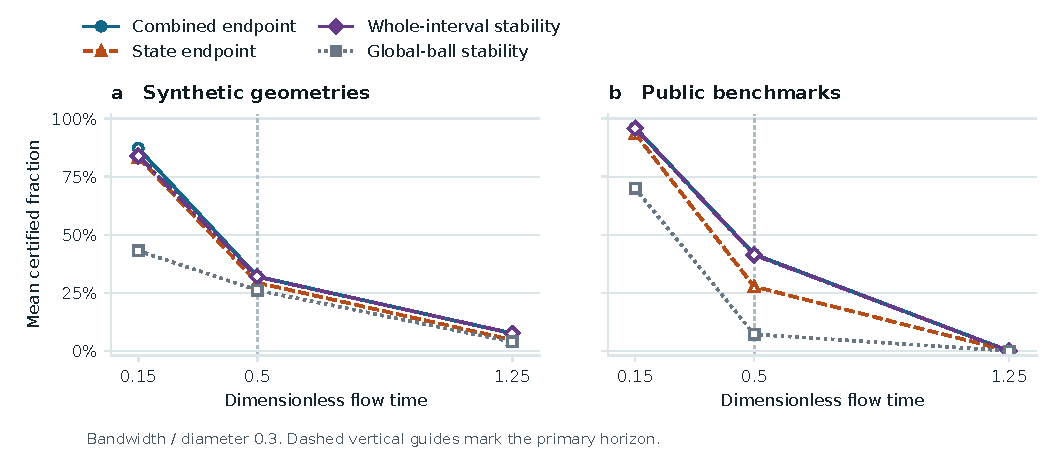
\includegraphics[width=\linewidth]{figures/certification.pdf}
\caption{Terminal-label and whole-interval coverage across the preregistered horizons. A terminal label can be certified after a return to the initial class. A stability certificate excludes any departure during the interval.}
\label{fig:certification}
\end{figure}

\subsection{A field-call saving can lose time}
The selective state-bound guard reduced field calls by 24.43\% on synthetic queries and 22.72\% on public queries, with no observed primary label mismatches to DOP853 (Table~\ref{tab:cost}). Its median batch latency ratios to unguarded RK4 were $1.32$ and $1.42$. The coverage and efficiency gates for a strict deployment advantage failed in both stages. Coverage is concentrated in easy regions. At the primary setting the combined diagnostic covered every separated-lobe query, whereas coverage on the open chains was 0.42\%. The guarded solver was faster than full RK4 in the lobe control and slower on the other primary families at their median settings.

The empirical triage policy gave a different fidelity--cost trade-off. The median latency ratios were $0.52$ and $0.69$, with zero synthetic disagreements in 51,840 primary query evaluations and one public disagreement in 1,889. Direct ETD1 readout was faster and disagreed on 637 and 25 of those evaluations. At $t=1.25$ and bandwidth ratio $0.30$, triage disagreed on 561 synthetic and 41 public evaluations. The shorter-horizon finding is therefore conditional on the tested setting. Triage is a fixed numerical heuristic without the guard's continuous-time guarantee. Query totals count repeated settings and held-out points used across gaps. They do not provide an independent-sample bound on triage error in new deployment domains.

\begin{table}[htbp]
\centering
\small
\caption{Primary numerical fidelity and cost. Latency ratios are medians of paired task-seed batch ratios versus fixed-step RK4. Disagreements compare each output with DOP853.}
\label{tab:cost}
\begin{tabular}{lrrrr}
\toprule
 & \multicolumn{2}{c}{Synthetic ($n=51{,}840$)} & \multicolumn{2}{c}{Public ($n=1{,}889$)}\\
Rule & Time ratio & Disagreements & Time ratio & Disagreements\\
\midrule
RK4 & 1.00 & 0 & 1.00 & 0\\
State-bound guard + RK4 & 1.32 & 0 & 1.42 & 0\\
One-step exponential Euler & 0.12 & 637 & 0.14 & 25\\
Projection triage + RK4 & 0.52 & 0 & 0.69 & 1\\
\bottomrule
\end{tabular}
\end{table}

\subsection{External class risk depends on the geometry and the underlying label law}
Transport improved balanced accuracy by 7.43 points on affine shells and reduced it by 4.77 on wavy shells. The paired largest-minus-smallest gap contrast in net harm averaged $+3.82$ points over the two shell families, with seed interval $[-4.68,+12.26]$. The shell-family point estimates were $+10.16$ on affine and $-2.52$ on wavy shells. At the primary setting the mean public decrease was $2.11$ points, with conditional seed interval $[1.11,3.28]$. These results did not establish a transferable law that widening the gap makes transport more harmful. They separate accurate identification of changed decisions from the weaker ability to predict the sign of the true-label effect.

In the known-law calibration, the symmetric binary tie was invariant and both coefficients were zero. The three nonzero cases checked both predicted coefficients to within 0.27\% relative error at the shortest measured horizon, $t=0.002$. Maximum absolute disagreement between direct Gaussian-CDF excess risk and localized quadrature was below $10^{-15}$. The solver displacement determined which pointwise decisions changed. The density contrast in each swept strip determined the much smaller classification regret (Figure~\ref{fig:oracle}). This calibration checks the specialization in Section~\ref{sec:bayes} under known Bayes orderings.

\begin{figure}[htbp]
\centering
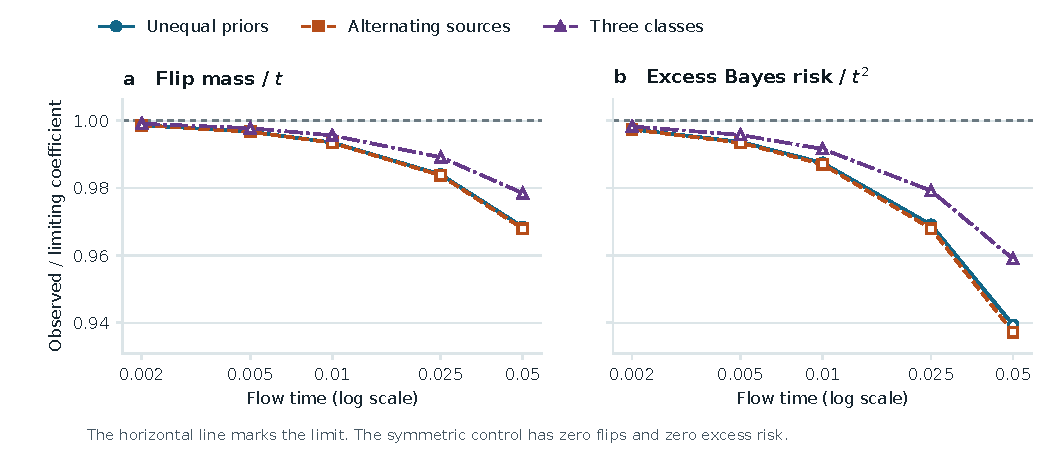
\includegraphics[width=\linewidth]{figures/oracle.pdf}
\caption{Known-law calibration. Normalizing the flip probability by $t$ and the excess Bayes risk by $t^2$ gives limits predicted from the same regular ties. The symmetric case is zero and is excluded from the ratios.}
\label{fig:oracle}
\end{figure}
